\chapter{Evaluación}
\label{cap:evaluacion}

En este capítulo se describe el proceso de evaluación de la aplicación que se ha llevado a cabo. Como ya se puso de manifiesto en el Plan de trabajo (ver Sección \ref{sec:planTrabajo}), la idea inicial era la de realizar una evaluación con usuarios finales y, preferiblemente, en la Facultad de Informática de la UCM, pues ese espacio es nuestro caso de estudio inicial. Debido a la crisis sanitaria y el estado de emergencia declarado en marzo de 2020 a causa de la COVID-19, no ha sido posible la ejecución de dicha evaluación. Sin embargo, conseguimos sobreponernos a este contratiempo y poner de manifiesto la flexibilidad de la aplicación mapeando otro edificio y realizando diversas pruebas sobre él. Este edificio no pudo ser otro que una vivienda. Cabe destacar que este no es el escenario ideal sobre el que se desplegaría una aplicación como Blind Bit, pues el espacio queda considerablemente reducido en comparación con el un edificio público como una facultad o museo, por ejemplo. A pesar de ello, permite probar el comportamiento de la aplicación en situaciones donde cierta aglomeración de \textit{beacons} es necesaria y poner a prueba el mapeo de un edifico con características distintas al ya planteado en la Sección \ref{sec:mapeo}. En las secciones que siguen se detalla cómo se ha llevado a cabo la adaptación tanto del plan de evaluación como el despliegue de la aplicación en este otro edificio.

En la Sección \ref{sec:adaptacionApp} se describen los pasos a seguir, tanto en el servidor (Sección \ref{sub:cambiosServidor_vivienda}) como en el cliente (Sección \ref{sub:cambiosCliente_vivienda}) para poder adaptar la aplicación al nuevo espacio. Por su parte, la Sección \ref{sec:objetivosEval} detalla los objetivos de la evaluación. Las pruebas que se llevaron a cabo a fin de valorar el cumplimiento de estos objetivos se exponen en la Sección \ref{sec:realizYresult} y las conclusiones finales de la evaluación pueden verse en la última sección (Sección \ref{sec:conclusionesEval}).


\section{Adaptación de la aplicación al nuevo edificio}
\label{sec:adaptacionApp}

En esta sección detallaremos los cambios que se han realizado para poder desplegar Blind Bit sobre la vivienda. Veremos tanto los cambios referentes al servidor (Sección \ref{sub:cambiosServidor_vivienda}) como al cliente (Sección \ref{sub:cambiosCliente_vivienda}). Hay que tener en cuenta que ninguno de estos cambios implica la modificación del código de la aplicación, pues esta se ha implementado de manera genérica para permitir su reutilización en nuevos espacios como el que se expone a continuación.

\subsection{Cambios en el servidor}
\label{sub:cambiosServidor_vivienda}

En la Sección \ref{sub:cambiosServidor} se exponen las claves para realizar el mapeo de un nuevo edificio. A continuación veremos cómo se han aplicado estas para el mapeo de la vivienda.


	
\begin{figure}[t!]
	\centering
	
	\subfloat[Mapeo de la planta baja de la vivienda]{
		\label{fig:mapeoCasaPBaja}
		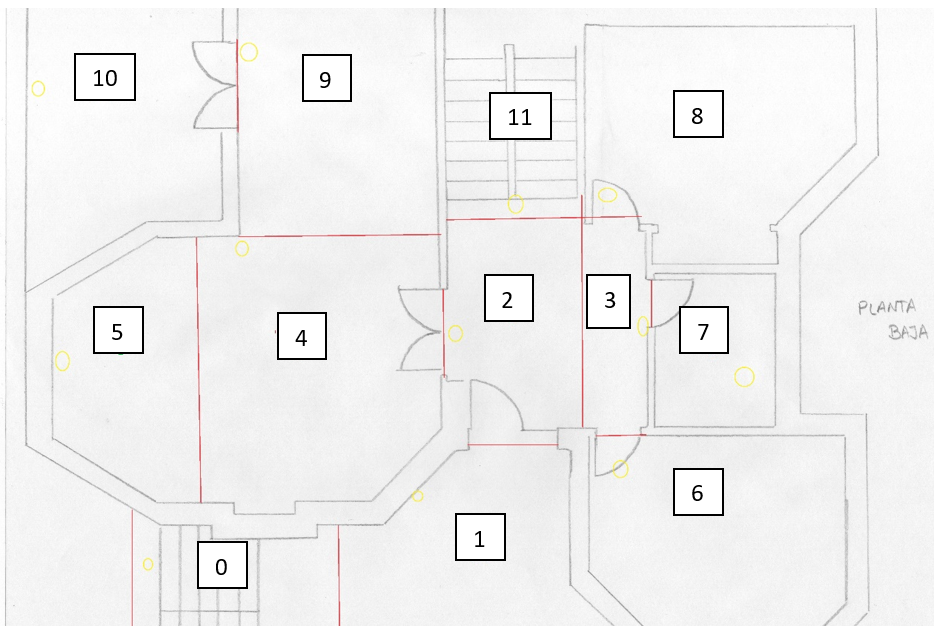
\includegraphics[width=0.8\textwidth]{Imagenes/Evaluacion/planoCasaPBaja}}
	
	\subfloat[Mapeo de la planta alta de la vivienda]{
		\label{fig:mapeoCasaPAlta}
		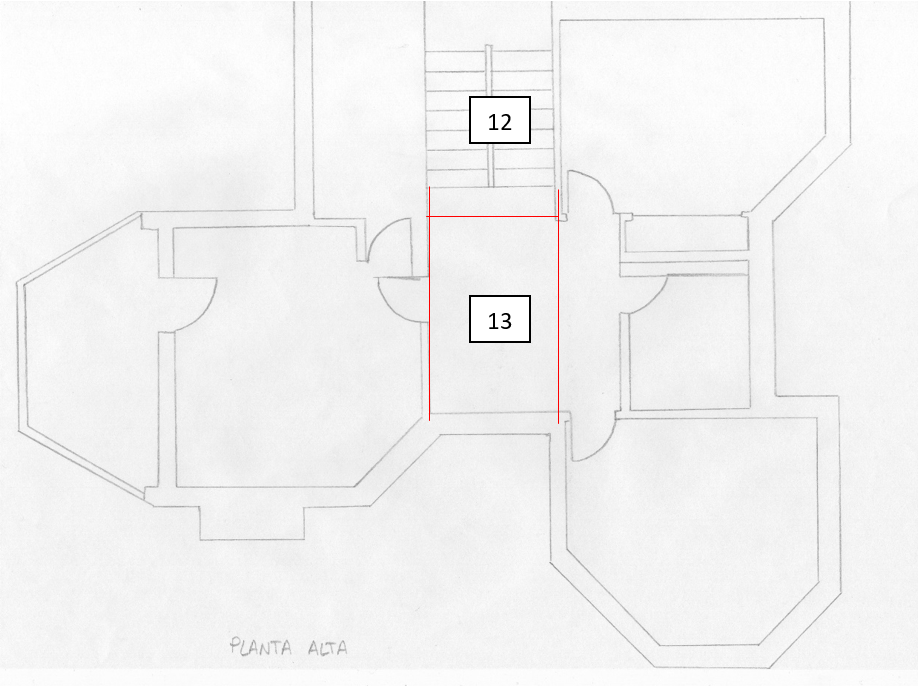
\includegraphics[width=0.8\textwidth]{Imagenes/Evaluacion/planoCasaPAlta}}\\
	
	\caption{Mapeo de la vivienda}
	\label{fig:mapeoCasa}
\end{figure}

\begin{enumerate}
	\item \textit{Características del edificio y necesidades del cliente:} El mapeo de una vivienda tiene ciertas particularidades que no se nos presentaron a la hora de mapear la Facultad de Informática de la UCM. Por un lado, las distancias se acortan, las distintas estancias, pasillos e intersecciones están mucho más cerca de lo que estarían en un edificio abierto al público, lo que implica que hay que tener más cuidado a la hora de posicionar los \textit{beacons}. Por otro lado, el número de puntos de interés es bastante más reducido y las rutas de puerta a puerta quedan demasiado simples a la hora de hacer una evaluación. Por esta razón, y a diferencia del trabajo realizado en la Facultad de Informática, en este caso sí hemos mapeado las distintas estancias, para añadir complejidad a la guía y que esta no se limite a ir por pasillos o recibidores.
	
	\item \textit{Trazado de los cuadrantes:} Para ello, lo primero que se ha hecho ha sido dividir el edificio en cada una de sus plantas y finalmente dividir estas en cuadrantes únicos. Buena parte de la decisión de la ubicación de las fronteras de los cuadrantes venía dada por la propia estructura del edificio, sus paredes y estancias. Sin embargo, no se debe olvidar que los cuadrantes solo pueden tener un punto de decisión y que no pueden colindar con más de un cuadrante por lado. Se puede ver el resultado del trazado de cuadrantes (rojo), cuyos identificadores son los números que aparecen sobre ellos, y la ubicación de los \textit{beacons} (amarillo) en la Figura \ref{fig:mapeoCasa}. En la Figura \ref{fig:mapeoCasaPBaja} vemos como hemos dividido la planta baja de la vivienda en 11 cuadrantes, siendo este último el que se corresponde con las escaleras que unen esta planta con el cuadrante 12 de la planta superior. El mapeo de la primera planta se encuentra en la Figura \ref{fig:mapeoCasaPAlta} que como vemos tiene la misma estructura que la planta inferior a excepción de la superficie que se corresponde con los cuadrantes $0$, $1$ y $10$ que desaparecen. Solo hemos incluido dos cuadrantes ya que la división es completamente análoga.	
	
	\item \textit{Información de los cuadrantes:} En este caso, la información adicional sobre los cuadrantes ha quedado reducida, limitándose a rellenar los campos correspondientes con datos aproximados\footnote{Tanto la información adicional, como los metros de cada cuadrante se corresponden con parámetros de prueba}. Esto se debe a que los objetivos de la evaluación (ver Sección \ref{sec:objetivosEval}) se enfocan al \textit{testeo} de la aplicación, rebajando peso a la parte de usabilidad, que no ha podido realizarse debido a las cuestiones sanitarias expuestas en la introducción. 
	
	\item \textit{Estructuración de los archivos:} Una vez mapeado el edificio, el siguiente paso ha sido estructurar la información en tres archivos XML que contienen los mismos campos descritos en la Sección \ref{sub:mapeo_xml}: uno de ellos que haga referencia al esqueleto del edificio y los otros dos que plasmen la información de cada una de las plantas. Además, se ha incluido el archivo \textit{destinos.json} (descrito en la Sección \ref{sub:func_servidor}) con las estancias que se han considerado destino y su cuadrante asociado.%En el Apéndice X podemos ver estos archivos XML.
\end{enumerate}


\subsection{Cambios en el cliente}
\label{sub:cambiosCliente_vivienda}

En la Sección \ref{sub:cambiosCliente} destacamos la poca dependencia al edificio que contiene el código referente al cliente. De hecho, vimos que bastaba con sustituir los nombres de los destinos en dos estructuras creadas en XML\footnote{Recordemos que la lista de destinos que se expone en las instrucciones de la aplicación y que se guarda en el mismo archivo (\textit{listasStringsApp.xml}) también debe ser modificada, en consonancia con la lista de destinos de la aplicación.}. En nuestro caso, esas estructuras tienen la siguiente forma: 

\lstinputlisting[language=XML]{Imagenes/Evaluacion/destinos_array_vivienda.xml}

\lstinputlisting[language=XML]{Imagenes/Evaluacion/destinosdinamicos_array_vivienda.xml}

Donde el número que acompaña a la estancia indica el cuadrante correspondiente a la misma.

\section{Objetivos de la evaluación}
\label{sec:objetivosEval}

Debido a la imposibilidad de realizar una evaluación con usuarios con discapacidad visual, nos vimos obligadas a reestructurar el \textit{modus operandi} de la evaluación de la aplicación. Concretamente, los objetivos cambiaron, centrándose en el funcionamiento de la misma y dando menos peso a la usabilidad, en la que los usuarios finales tienen un papel decisivo. De esta manera, se decidió establecer cuatro objetivos claros que presentamos a continuación:

\begin{enumerate}
	
	\item \textit{Resolución del problema del posicionamiento:} Una de las funcionalidades principales de la aplicación es, sin duda, la correcta ubicación del usuario. Para ello es necesario que el \textit{beacon} más cercano al usuario sea detectado como el más cercano por la aplicación (ver Sección \ref{sub:func_cliente}). De esta tarea depende no solo el inicio de la ruta sino el seguimiento de toda ella, pues en todo momento debemos conocer el cuadrante donde se encuentra el usuario para que la aplicación pueda responder en consecuencia. Una mala ubicación del usuario podría provocar que el usuario se pierda debido a indicaciones que no corresponden con su posición o, en casos más graves, el tropiezo del usuario con un obstáculo del que no ha sido advertido.
	
	Cabe destacar que en el posicionamiento influye no solo la correcta implementación del código, sino también la ubicación de los \textit{beacons}, que debe adaptarse a las necesidades específicas de cada edificio. 
	
	\item \textit{Generación de instrucciones correctas:} Teniendo en cuenta la ubicación del usuario y el camino que ha seguido, es primordial que la aplicación sea capaz de generar instrucciones correctas. Tanto los giros como la señalización de puntos de interés, como los ascensores o el destino, debe corresponderse con la ubicación real de estos, tal y como se establece en los archivos XML (ver Sección \ref{sub:mapeo_xml}).
	
	\item \textit{Precisión de las instrucciones:} Además de que las instrucciones sean correctas, hay que evaluar que el usuario las recibe en el momento adecuado. Esto está claramente relacionado con el posicionamiento, pues el momento de indicación de la ruta se basa en cuándo el usuario llega a un determinado cuadrante. Sin embargo, se debe prestar especial atención a las posibles variaciones que pueden darse (una instrucción puede darse con cierta antelación o, por el contrario, una vez pasado el punto óptimo) y evaluar si esa flexibilidad es asumible para el usuario.
	
	\item \textit{Ejecución correcta en caso de usuario perdido:} Este es un punto importante, pues no debemos asumir que el usuario va a seguir siempre la ruta correcta, y puede ocurrir que por diversos motivos (una distracción, un obstáculo o el propio fallo de la aplicación) el usuario se desvíe de esta ruta. En ese caso no solo se debe identificar el problema sino también saber reconducir al usuario al destino deseado. 
		
\end{enumerate}


\section{Realización y resultados de la evaluación}
\label{sec:realizYresult}

En esta sección se exponen las pruebas realizadas para evaluar la aplicación, así como su posterior análisis. A pesar de que el espacio con el que se cuenta para realizar estos ensayos no presenta tantas posibilidades como la Facultad de Informática de la UCM\footnote{Es un espacio más reducido, con menos intersecciones, puntos de interés, obstáculos y tránsito de gente.}, estos han sido diseñados de tal manera que se cubran la mayor cantidad posible de casos, con la finalidad de detectar no solo posibles errores sino también confirmar que la aplicación es capaz de adaptarse a un nuevo espacio y funcionar de la manera esperada. En lo que sigue, asumiremos que \textit{beacon$X$} es el \textit{beacon} asociado al cuadrante $X$ y que la ubicación del punto de interés de cada cuadrante corresponde con la ubicación del \textit{beacon} siempre y cuando no se indique expresamente. 

\subsection{ Pruebas de seguimiento de la ruta}
En esta sección se detallan las pruebas realizadas asumiendo que el usuario no va a salir de la ruta. Sin embargo, algunas de ellas están diseñadas para reproducir situaciones extremas como la pérdida de un \textit{beacon} o rutas potencialmente complicadas.


\subsubsection{Ruta del cuadrante $0$ al cuadrante $10$}
\label{subsub:0al10}
La primera ruta de la evaluación consiste en realizar la ruta desde el cuadrante $0$ hasta el cuadrante $10$ sin salir de la ruta. Se ha comenzado por esta porque es una de las rutas más largas y con más giros, de esta manera se pueden comprobar diversos comportamientos de la aplicación a la vez. La Figura \ref{fig:del0al10} ilustra el trazado de la ruta.


\subsubsection*{Objetivos de la prueba}

Se quiere comprobar el correcto funcionamiento de los siguientes puntos:
\begin{itemize}
	
	\item Funcionamiento de los distintos métodos de entrada para introducir el destino (teclado, botón y micrófono).
	
	\item El posicionamiento del usuario en un cuadrante se realiza de manera correcta por medio del \textit{beacon} más cercano. 
	
	\item En base al posicionamiento y la ruta que sigue el usuario las instrucciones que se le indican son correctas. 
	
	\item Las instrucciones se reflejan en la pantalla (la última instrucción siempre queda visible, el resto se pueden recuperar haciendo \textit{scroll} hacia arriba) y se reproducen mediante voz (solo la última instrucción).
	
	\item La información no verbal, como el sonido \textit{check} y las vibraciones asociadas a los giros y llegada al destino, están correctamente implementadas. Para las vibraciones se comprueba que son lo suficientemente distintas para que el usuario sea capaz de distinguirlas.
	
	\item Las instrucciones se indican al usuario en el momento adecuado. 
\end{itemize}

\begin{figure}[t]
	\centering
	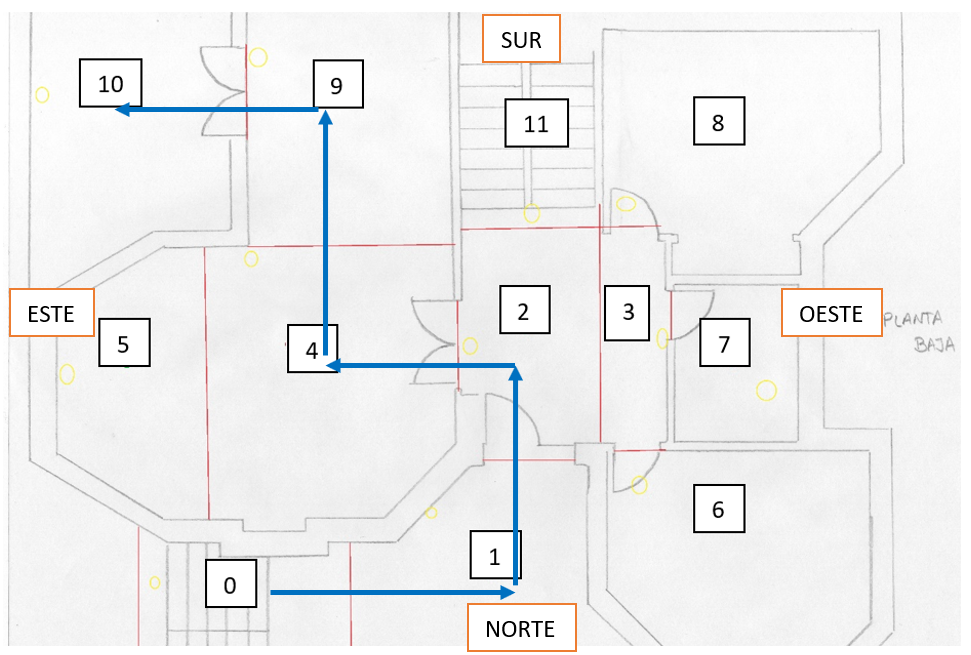
\includegraphics[width=0.8\textwidth]{Imagenes/Evaluacion/del0al10}
	\caption{Ruta del cuadrante $0$ al $10$.}
	\label{fig:del0al10}
\end{figure}

\subsubsection*{Comportamiento esperado}

Al comienzo de la prueba la aplicación debe reconocer el destino \textit{estancia $10$} por cualquiera de sus métodos de entrada (teclado, botón y micrófono). Una vez reconocido, la aplicación debe mostrar la pantalla de ruta (ver Figura \ref{fig:interfaz}) y, tras pulsar \textit{Iniciar ruta}, se debe comenzar a guiar al usuario habiendo establecido que su posición inicial es el cuadrante $0$. Cuando el usuario cumpla con la primera instrucción y llegue al cuadrante $1$, esta debe emitir el sonido \textit{check} (esto mismo debe repetirse cada vez que se completa una instrucción). La instrucción correspondiente al cuadrante $1$ debe ser proporcionada al usuario hacia la mitad del cuadrante, de tal manera que sepa que debe completar unos metros antes de girar. En el caso del cuadrante $2$ (y de todos aquellos donde el giro sea inmediato, el resto) la instrucción debe darse con cierta anterioridad al giro, para evitar que el usuario pase la intersección (esto tiene que ver con el posicionamiento de los \textit{beacons}), y la dirección de giro debe ser la correcta. Durante toda la ruta se comprueba que en las instrucciones de giro el dispositivo móvil vibra acorde a la dirección de giro, una vibración larga cuando se trata de un giro a la izquierda y dos cortas cuando es un giro a la derecha. Al llegar al destino se comprueba que la vibración es la adecuada (tres vibraciones cortas) y que se indica al usuario la posición del punto de interés final, en este caso a la derecha (se estableció que el punto de interés del cuadrante $10$ está al sur).

Durante el trayecto las instrucciones deben mostrarse por pantalla y ser reproducidas por voz de la manera descrita en los objetivos.

\subsubsection*{Comportamiento durante la prueba}
 
El recorrido se realizó hasta en cinco ocasiones a fin de encontrar irregularidades durante el transcurso de la ruta. 


Las Instrucciones generadas para cada cuadrante fueron las siguientes\footnote{La distancia estimada de cada cuadrante ha sido 5.0 metros.}:

\begin{itemize}
	\item Cuadrante 0: \textit{Continúa recto 5.0 metros. Luego gira a la izquierda.}
	
	\item Cuadrante 1: \textit{Gira a la izquierda. Luego continúa recto 5.0 metros.}
	
	\item Cuadrante 2: \textit{Gira a la izquierda. Luego continúa recto 5.0 metros.}
	
	\item Cuadrante 4: \textit{Gira a la derecha. Luego continúa recto 5.0 metros.}
	
	\item Cuadrante 9: \textit{Gira a la izquierda. Luego continúa recto 5.0 metros.}
	 
	\item Cuadrante 10: \textit{Tu destino está a la derecha.}
\end{itemize}

A continuación se presentan los puntos a destacar de las distintas pruebas realizadas.


\begin{itemize}
	
	\item El primer punto a destacar es que el reconocimiento del destino ``estancia $10$'' fue reconocido por medio del teclado, el botón y el micrófono. Tan solo en una ocasión el micrófono reconoció ``instancia $10$'' e indicó al usuario que se trataba de un destino no válido. Mediante el teclado se introdujo en la barra de búsqueda este mismo texto ``instancia $10$'' para comprobar el comportamiento. En este caso también se indicó al usuario que no era un destino válido. 
	
	Cuando el destino se reconoce con éxito, la aplicación despliega de manera automática la pantalla de ruta y espera a que el usuario pulse \textit{Iniciar ruta}. 
	
	\item El posicionamiento inicial del usuario en el cuadrante $0$ se realizó correctamente en cada una de las cinco pruebas.
	
	\item Las instrucciones generadas por la aplicación son correctas. Cuando el usuario no tiene que realizar un cambio de dirección de manera inmediata, primero se le indican los metros que debe continuar en esa dirección y luego hacia dónde tiene que girar (caso del cuadrante $0$). En caso de que el usuario deba cambiar la dirección de su marcha, primero se indica la dirección de giro y luego los metros que debe continuar en esa dirección (resto de cuadrantes de la ruta). Además, las instrucciones se muestran por pantalla y se indican mediante voz de la manera esperada.
	
	\item En la mayor parte de los casos, las instrucciones se indican al usuario en el momento adecuado. Sin embargo, en dos ocasiones las instrucciones correspondientes a los cuadrantes $1$ y $2$ se dieron demasiado pronto. 
	
	\item Las vibraciones asociadas a los giros y a la llegada del destino son lo suficientemente distintas para que el usuario pueda distinguirlas.
	
	\item En una de las ocasiones el \textit{beacon} asociado al cuadrante $4$ no fue detectado por la aplicación, provocando la pérdida de esa instrucción. En las pruebas siguientes se detalla el comportamiento de la aplicación en este caso (ver Secciones \ref{subsub:0al10sin4} y \ref{sub:usuarioPerdido}).
	
	\item Una vez se ha llegado al destino, la posición del punto de interés se indica correctamente en función de la dirección desde la que proviene del usuario, ``su destino está a la derecha''. Además, se emiten tres vibraciones cortas, que hacen notar al usuario que es la última instrucción de la ruta.
	
\end{itemize}

\subsubsection*{Conclusiones}

Como hemos podido comprobar, el funcionamiento del código de la aplicación es correcto, puesto que las instrucciones generadas (verbales y no verbales) son las esperadas. Sin embargo, se ha detectado un problema de detección de \textit{beacons} en el punto con más aglomeración de la ruta, el comprendido por los cuadrantes $1$, $2$ y $4$. Llama la atención la pérdida de la instrucción correspondiente al \textit{beacon$4$}, lo que sugiere que la aplicación no lo ha detectado como \textit{beacon} más cercano cuando debería. Tras observar la ubicación de los \textit{beacons}, lo más probable es que se detectara el \textit{beacon$1$} o el \textit{beacon$2$} como los más cercanos. En la siguiente prueba abordamos este problema con más detalle. 

El hecho de que las instrucciones correspondientes a los cuadrantes $1$ y $2$ se dieran con demasiada antelación puede deberse a que el \textit{beacon} del cuadrante $1$ está situado en una terraza, separado del $0$ por una puerta de cristal. La instrucción de giro se dio nada más pasar esa puerta, lo que implica demasiada antelación al giro. Una vez que se avanza hacia la puerta que separa los cuadrantes $1$ y $2$, la distancia que hay entre ellos es reducida, es por ello que el \textit{beacon$2$} se establece como el más cercano rápidamente, y provoca que la aplicación indique la instrucción de giro un metro antes de encontrar la puerta entre los cuadrantes $2$ y $4$.


\subsubsection{Posicionamiento inicial en el cuadrante $1$}
\label{subsub:pos1}

En este caso lo que se pone a prueba es el posicionamiento inicial del usuario en el cuadrante $1$. La razón por la cual se decidió hacer esta prueba fue la pérdida de la instrucción del cuadrante $4$ en el caso anterior (Sección \ref{subsub:0al10}). Esa prueba indica que el \textit{beacon$4$} no se detectó como el más cercano cuando el usuario se encontraba en este mismo cuadrante, sugiriendo que el \textit{beacon} que se detectaba como más cercano debía ser el $1$ o el $2$, por la ubicación de los \textit{beacons} (ver Figura \ref{fig:posic1}).


\subsubsection*{Objetivos de la prueba}

\begin{itemize}
	\item Establecer de manera correcta el posicionamiento inicial del usuario en el cuadrante $1$.
	
	\item Como la ruta no se desarrolla hasta el final, se comprueba el correcto funcionamiento del botón \textit{Finalizar ruta} (ver Figura \ref{fig:interfaz}).
\end{itemize}


\begin{figure}[t]
	\centering
	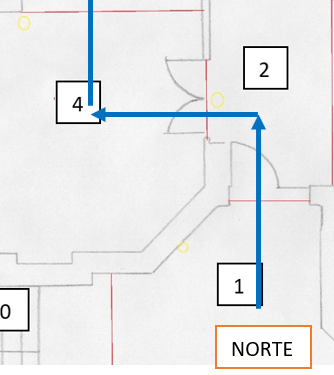
\includegraphics[width=0.5\textwidth]{Imagenes/Evaluacion/posic1}
	\caption{Problema del posicionamiento en el cuadrante $1$.}
	\label{fig:posic1}
\end{figure}

\subsubsection*{Comportamiento esperado}

La prueba comienza en el cuadrante $1$. Tras introducir el destino ``estancia 10'' y haber pulsado \textit{Iniciar ruta} en la pantalla de ruta, la primera instrucción de la aplicación debe ser la correspondiente a este cuadrante (Continuar recto y luego girar a la izquierda). En este caso no se continuó la prueba hasta el destino para no repetir lo realizado anteriormente. Por esta razón, una vez comprobado el posicionamiento se fuerza la finalización de la ruta mediante el botón \textit{Finalizar ruta}. Como hay una ruta iniciada este debe mostrar un cuadro de texto preguntando al usuario confirmación para la finalización de la ruta y la vuelta a la pantalla anterior. En caso de aceptar se vuelve atrás. En caso de cancelar, la ejecución de la aplicación continúa como hasta entonces, permitiendo que el usuario siga recibiendo instrucciones sin necesidad de pulsar ningún otro botón.


\subsubsection*{Comportamiento durante la prueba}

Se hicieron cinco pruebas y se pudo comprobar que en dos ocasiones este posicionamiento no se realizó de manera correcta. En una de ellas el \textit{beacon} más cercano inicial detectado por la aplicación fue el $4$ y en la otra el $2$.

El comportamiento del botón \textit{Finalizar ruta} fue el esperado. Se probaron tanto la opción \textit{Aceptar} como \textit{Cancelar} del \textit{pop-up}.


\subsubsection*{Conclusiones}

De esta prueba destacamos la importancia de que los \textit{beacons} estén lo suficientemente separados y, en la medida de lo posible, en las mismas condiciones (ver Sección \ref{sec:medicionesbeacons}). En este caso lo que ha ocurrido es que la separación entre los \textit{beacons} $1$ y $4$ está delimitada físicamente por una ventana, cuyo grosor es más fino que el de una pared o cierto mobiliario. Esto, sumado a que la distancia estimada por la aplicación presenta ciertos picos al principio como se vio en la Sección \ref{sub:pruebasCuadrantesv1}, provoca que el \textit{beacon} que se lee como más cercano no sea el correcto. El hecho de que en esta zona del mapa no se identifique de manera adecuada el \textit{beacon} más cercano puede dar explicación a la pérdida del \textit{beacon$4$} en la sección anterior (Sección \ref{subsub:0al10}). La posible razón por la cual el \textit{beacon$2$} también fuera detectado como el más cercano está expuesta en la prueba anterior.


\subsubsection{Ruta del cuadrante $0$ al cuadrante $10$, eliminando el \textit{beacon} del cuadrante $4$}
\label{subsub:0al10sin4}

En este caso se ha vuelto a repetir la ruta del cuadrante $0$ al $10$ con la particularidad de que el \textit{beacon$4$} se eliminó de la ruta. Sin embargo, no provocamos la situación de que el usuario se saliera de la ruta (como sería lógico en esta situación, pues la instrucción de giro del cuadrante $4$ se pierde), continuamos por el cuadrante $9$ (ver Figura \ref{fig:del0al10sin4}, donde la instrucción perdida corresponde con la flecha discontinua). 

\subsubsection*{Objetivo de la prueba}

\begin{itemize}
	\item Comprobación del correcto funcionamiento de la aplicación cuando no se percibe la llegada del usuario a un cuadrante pero este continua en la ruta en un cuadrante más avanzado.
\end{itemize}


\begin{figure}[t]
	\centering
	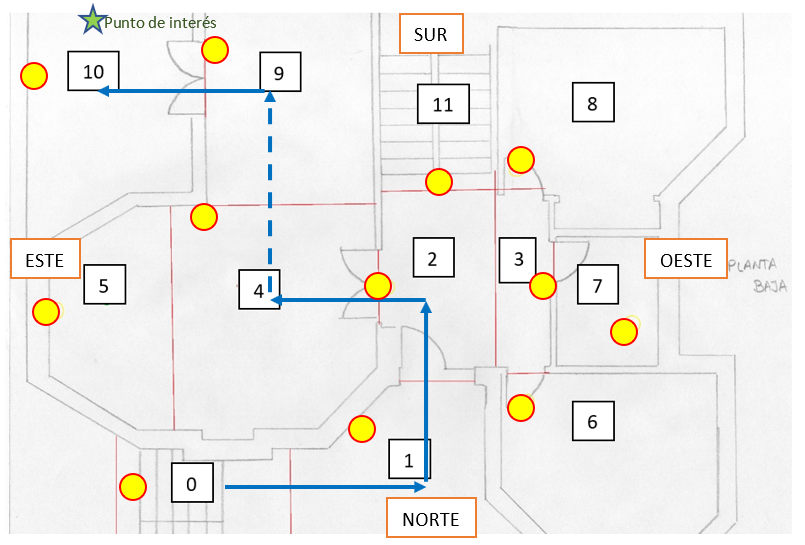
\includegraphics[width=0.8\textwidth]{Imagenes/Evaluacion/del0al10sin4}
	\caption{Ruta del cuadrante $0$ al $10$, eliminando el \textit{beacon$4$}.}
	\label{fig:del0al10sin4}
\end{figure}

\subsubsection*{Comportamiento esperado}

El comportamiento de la aplicación debe ser el descrito en la Sección \ref{subsub:0al10} hasta llegar al cuadrante $4$. En ese momento la aplicación espera a que el \textit{beacon} más cercano sea el \textit{beacon$4$} durante cierto tiempo para dar la instrucción correspondiente (ver Seguimiento de la ruta en la Sección \ref{sub:func_cliente}). Este tiempo debe aproximarse al tiempo transcurrido en ir desde el cuadrante $2$ al $9$. Una vez que el usuario está en el cuadrante $9$ y la aplicación ha identificado que, a pesar de que el usuario no ha notificado la llegada al cuadrante $4$, se encuentra en un cuadrante que forma parte de la continuación de la ruta (no se ha perdido), debe indicarle la instrucción correcta atendiendo al camino que lleva recorrido (se supone que ha seguido la ruta), en este caso un giro a la izquierda. El final de la ruta debe ser el habitual: tres vibraciones cortas y la indicación de la posición del punto de interés, en este caso a la derecha como en la Sección \ref{subsub:0al10}.


\subsubsection*{Comportamiento durante la prueba}

Nos centraremos en el comportamiento transcurrido entre los cuadrantes $2$ y $9$, pues el resto ya ha sido comentado en \ref{subsub:0al10}. Una vez recibida la instrucción de giro a la izquierda del cuadrante $2$, se simuló la recepción de la instrucción de giro a la derecha del cuadrante $4$. Esta nunca llegó a recibirse, pues el \textit{beacon$4$} no estaba en su posición. Cuando se llegó al cuadrante $9$ se esperaba a la instrucción de giro a la izquierda correspondiente pero esta se emitió con bastante retraso. Esto se debe a que el umbral de la variable \textit{numPasosPerdidos}, que identifica el momento en el que el usuario puede haberse perdido (ver Seguimiento de la ruta en la Sección \ref{sub:func_cliente}), es demasiado elevado para este edificio, donde las distancias entre \textit{beacons} son pequeñas. Para solventar este problema, lo que se hizo fue reducir este umbral de 10 a 5, y de esta manera la instrucción se recibió en el momento adecuado. Como la aplicación sigue con la ejecución esperada desde el cuadrante $9$ no se percibe la falta del \textit{beacon$4$}, evitando que el usuario sea notificado sin necesidad.


\subsubsection*{Conclusiones}

De esta prueba destacamos la necesidad de ajustar los umbrales de la variable \textit{numPasosPerdidos} a las características del edificio. De esta manera podemos evitar que el usuario continúe por una ruta equivocada durante demasiado tiempo o, como en este caso, que reciba confirmación de su trayecto demasiado tarde. En la prueba siguiente veremos otro caso donde se pone de manifiesto la importancia de este ajuste.


\subsubsection{Ruta del cuadrante $1$ al cuadrante $5$, eliminando el \textit{beacon} del cuadrante $2$}
\label{subsub:1al5sin2}

Este caso está relacionado con el anterior, pues la base del caso de estudio es la misma: la pérdida de un \textit{beacon}. Sin embargo, en esta prueba se pone de manifiesto la ventaja de la anticipación de instrucciones, pues favorecen que, en caso de que un \textit{beacon} no sea detectado, el usuario permanezca en la ruta y llegue a su destino, aun cuando ese \textit{beacon} corresponda a una intersección. La ruta que se va a probar es la comprendida entre los cuadrantes $1$ y $5$, con la particularidad de que el \textit{beacon2} se ha eliminado. La Figura \ref{fig:del1al5sin2} ilustra este recorrido, donde la instrucción perdida se representa con una flecha discontinua.

\subsubsection*{Objetivo de la prueba}

Como el comportamiento de la aplicación en caso de falta de detección de un \textit{beacon} y seguimiento de la ruta se ha abordado en la Sección \ref{subsub:0al10sin4}, se ha incluido en esta ruta el \textit{testeo} de otra funcionalidad de la aplicación. 

\begin{itemize}
	\item Comprobación del correcto funcionamiento de la aplicación cuando no se percibe la llegada del usuario a un cuadrante pero este continua en la ruta en un cuadrante más avanzado.
	
	\item Comprobación del correcto funcionamiento del \textit{modo mute} de la aplicación. Esta funcionalidad se corresponde con la descripción del botón en forma de altavoz en la pantalla de ruta (ver Sección \ref{sub:diseño}). 
\end{itemize}

\begin{figure}[t]
	\centering
	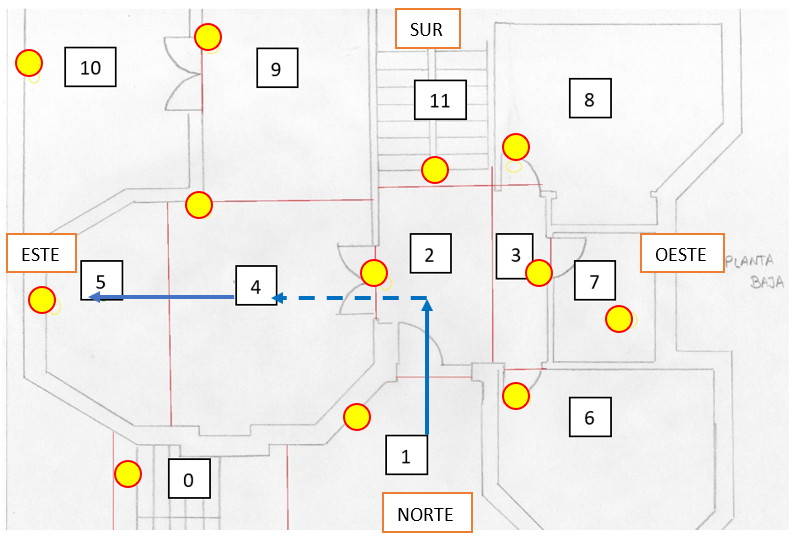
\includegraphics[width=0.8\textwidth]{Imagenes/Evaluacion/del1al5sin2}
	\caption{Ruta del cuadrante $1$ al $5$, eliminando el \textit{beacon$2$}.}
	\label{fig:del1al5sin2}
\end{figure}

\subsubsection*{Comportamiento esperado}

El inicio de la prueba debe ser el descrito en el comportamiento esperado de la Sección \ref{subsub:pos1}. Una vez resuelto el posicionamiento del cuadrante $1$, la aplicación debe indicar al usuario que avance unos metros y luego gire a la izquierda. En este caso el usuario no va a recibir la confirmación de giro correspondiente al cuadrante $2$, porque ese \textit{beacon} se ha eliminado. Sin embargo, para esta prueba, vamos a suponer que el usuario continúa la ruta por el cuadrante $4$. Cuando el usuario llega a la mitad del cuadrante $4$, se le debe indicar que continúe recto. Por último, en las inmediaciones del cuadrante $5$ se debe finalizar con tres vibraciones cortas y la indicación de que el destino se encuentra delante (en este caso la posición del punto de interés del cuadrante $5$ es en el este).

Como se ha establecido en los objetivos de esta prueba, el modo silencio de la pantalla de ruta va a estar activado, lo que significa que ninguna instrucción debe emitirse por voz. Todas ellas deben ser leídas a través de la pantalla sin necesidad de hacer \textit{scroll}, pues siempre debe mostrarse la última instrucción escrita a pesar de que las instrucciones anteriores quedan en la parte superior a modo de registro. 


\subsubsection*{Comportamiento durante la prueba}

El comportamiento de la aplicación es el esperado. Las instrucciones generadas fueron las siguientes: 


\begin{itemize}
	\item Cuadrante 1: \textit{Continúa recto 5.0 metros. Luego gira a la izquierda.}
	
	\item Cuadrante 2: \textit{Gira a la izquierda. Luego continúa recto 10.0 metros.} (Instrucción perdida, no se mostró al usuario).
	
	\item Cuadrante 4: \textit{Continúa recto 5.0 metros.}
	
	\item Cuadrante 5: \textit{Tu destino está delante.}
	
\end{itemize}


Sin embargo, se ha apreciado un ligero retraso en la llegada de la instrucción del cuadrante $4$. 

 
\subsubsection*{Conclusiones}

Este caso es interesante, pues, a pesar de que se ha eliminado uno de los \textit{beacons} correspondientes a una intersección, la información de giro del cuadrante $2$ no se pierde. Esto se debe a que, como la aplicación es capaz de avisar de los cambios de dirección con antelación, en el cuadrante $1$ ya se indica al usuario que, tras avanzar unos metros, debe girar a la izquierda. Bien es cierto que se pierde precisión, pues el usuario no percibe la instrucción de giro en el momento en el que debe realizarse, ni la confirmación sonora y vibración asociada a esta. Sin embargo, el hecho de que se den instrucciones por adelantado favorece que el usuario permanezca en la ruta aun cuando alguna instrucción se pierda. 

Particularmente para esta ruta, el giro del cuadrante $2$ es el único que hay que realizar y, debido a esto, es más fácil que el usuario no se pierda. En caso de que el destino hubiera sido el cuadrante $10$, el ajuste del umbral de \textit{numPasosPerdidos} es esencial, pues un umbral muy alto provocaría que el usuario no hubiera llegado a recibir la instrucción de giro a la derecha del cuadrante $4$. Esto se debe a que la aplicación necesita un tiempo (llegar a un número de pasos perdidos) para decidir si el usuario se ha perdido. De esta manera, cuando el usuario llega al cuadrante $4$ la aplicación sigue a la espera del cuadrante $2$ (el umbral de \textit{numPasosPerdidos} es demasiado alto, ver funcionamiento en la Figura \ref{fig:diag_clienteSeguimientoRuta}). Esto implica que el usuario se salga de la ruta. Abordaremos este caso más adelante, en la Sección \ref{sub:usuarioPerdido}.


\subsubsection{Ruta del cuadrante $1$ al cuadrante $13$}
\label{subsub:del1al13}

En este caso lo que se quería evaluar eran las instrucciones referentes al cambio de planta. Como ya se comentó en la Sección \ref{sub:cambiosServidor}, el código asume que los cambios de planta se realizan por medio de ascensores. Esta información se ha ignorado en esta ocasión, pues solo se disponía de escaleras. La ruta que se prueba es la comprendida entre los cuadrantes $1$ y $13$ (ver Figura \ref{fig:del1al13}).

\subsubsection*{Objetivos de la prueba}

Como las funcionalidades asociadas a las instrucciones de la ruta han sido \textit{testeadas} en pruebas anteriores, se incluye en esta prueba la comprobación de los dos únicos botones de la pantalla de ruta que quedaban por probar.

\begin{itemize}
	\item Correcto funcionamiento de la aplicación cuando la ruta está formada por cuadrantes de distintas plantas. 
	
	\item Correcto funcionamiento del botón \textit{Repetir instruccción}.
	
	\item Correcto funcionamiento del botón \textit{Instrucciones detalladas.}
\end{itemize}

\begin{figure}[t]
	\centering
	
	\begin{tabular}{cc}
		\subfloat[Ruta del cuadrante $1$ al $11$ en la planta baja de la vivienda.]{
			\label{fig:del1al11}
			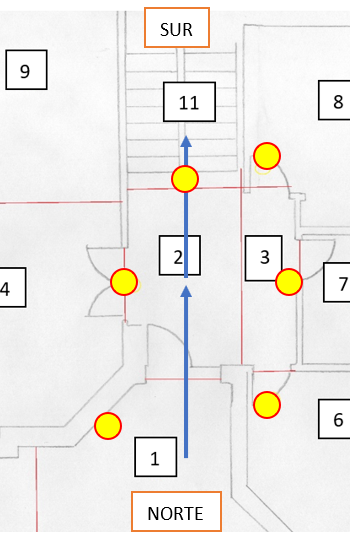
\includegraphics[width=0.5\textwidth]{Imagenes/Evaluacion/del1al13a}}
		& \subfloat[Ruta del cuadrante $12$ al $13$ en la planta alta de la vivienda.]{
			\label{fig:del12al13}
			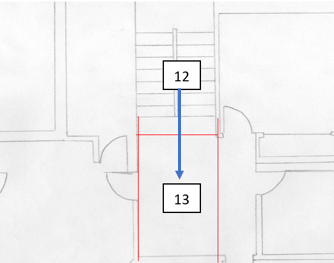
\includegraphics[width=0.5\textwidth]{Imagenes/Evaluacion/del1al13b}}\\
	\end{tabular}
	\caption{Ruta del cuadrante $1$ al $13$.}
	\label{fig:del1al13}
\end{figure}

\subsubsection*{Comportamiento esperado}

La aplicación debe reconocer el destino ``estancia 13'' por cualquiera de sus métodos de entrada (teclado, botón y micrófono). Una vez reconocido y tras pulsar \textit{Iniciar ruta} se debe recibir la primera instrucción, correspondiente al cuadrante $1$. Esta instrucción debe indicar al usuario que continúe recto los metros estimados hasta las escaleras. En el cuadrante $2$ la instrucción debe ser la misma pero el número de metros debe haberse reducido al estimado desde ese cuadrante a las escaleras. Si la funcionalidad instrucciones detalladas está activada, la aplicación debe advertir de los ascensores del siguiente cuadrante. Una vez llegamos a cuadrante $11$ se debe indicar al usuario en qué posición se encuentran, en este caso delante, y la planta a la que se debe dirigir, acompañado de la acción de subida o bajada, en este caso ``sube a la planta 1''. Una vez se ha llegado al cuadrante $12$, la aplicación debe reconocer la nueva posición del usuario (este se encontrará mirando hacia la puerta del ascensor) e indicarle la instrucción adecuada, ``continua recto'' en esta ocasión. Por último, la llegada al cuadrante $13$ debe realizarse de la manera ya descrita, con tres vibraciones cortas y la indicación de la oposición del punto de interés. Como se estableció que la posición de este era norte, debe ser ``su destino está delante''. 

Durante la ruta, si el modo instrucciones detalladas está activado, el usuario debe recibir tras cada instrucción la información adicional del cuadrante siguiente en la ruta. Por el contrario, si está desactivada no se debe recibir esta información. El botón \textit{Repetir instrucción} debe mostrar en pantalla y reproducir la ultima instrucción que se le ha dado al usuario cada vez que se pulsa. 


\subsubsection*{Comportamiento durante la prueba}

El comportamiento durante el inicio de la aplicación fue el esperado, los metros que había que recorrer desde el cuadrante $1$ a las escaleras se fueron reduciendo hasta llegar a ese punto. De la llegada al cuadrante $11$ destacamos que la instrucción correspondiente a este cuadrante tardó unos segundos más de lo esperado. Sin embargo, en el cuadrante $12$ se recibió en el momento oportuno (justo antes de llegar al final de las escaleras). La llegada al cuadrante $13$ también fue la esperada. Las instrucciones generadas fueron:

\begin{itemize}
	\item Cuadrante 1: \textit{Continúa recto 10.0 metros.}
	
	\item Cuadrante 2: \textit{Continúa recto 5.0 metros.} 
	
	\item Cuadrante 11: \textit{El ascensor está delante. Sube a la planta 1.}
	
	\item Cuadrante 12: \textit{Continúa recto 5.0 metros para salir de la zona de ascensores.}
	
	\item Cuadrante 13: \textit{Tu destino está delante.}
	
\end{itemize}

El inicio de la ruta se hizo con el modo instrucciones detalladas activado, mientras que el final (a partir del cuadrante $12$) con esta funcionalidad desactivada. El comportamiento en ambos casos fue el descrito como esperado. Así mismo, en dos ocasiones se pulsó el botón \textit{Repetir instrucción}, una antes de llegar al cuadrante $11$, cuando todavía no se había recibido la instrucción asociada a este, y otra justo al recibir la instrucción del cuadrante $12$. Esto desencadenó la reproducción y escritura en pantalla de la última instrucción que se había recibido, como estaba establecido. 

\subsubsection*{Conclusiones}


De la ruta desde el cuadrante $1$ al $13$ destacamos un punto importante, que es la anticipación de los ascensores en el cuadrante $2$ gracias a la información adicional, si la funcionalidad instrucciones detalladas está activada. Esto advierte al usuario con antelación de la necesidad de tomar un ascensor. El hecho de que la instrucción del cuadrante $11$ haya tardado en llegar puede deberse a que el \textit{hall} de la planta baja es una zona con alta concentración de \textit{beacons}, lo que provoca que la estimación del \textit{beacon} más cercano tarde en hacerse correctamente. 

\subsubsection{Ruta del cuadrante $13$ al cuadrante $8$}
\label{subsub:13al8}

La finalidad de esta ruta es, principalmente, comprobar el comportamiento de la aplicación en el \textit{hall} de la planta baja, así como el cambio de planta inverso. La ruta determinada para hacer esta prueba comienza en el cuadrante $13$ y finaliza en el $8$ (ver Figura \ref{fig:del13al8}). Como puede verse en la Figura \ref{fig:del11al8}, la disposición de los cuadrantes obliga al usuario a realizar dos giros a la izquierda para poder entrar al cuadrante $8$. Esto a simple vista puede resultar un poco tedioso puesto que si olvidamos por un momento la estructura de cuadrantes la ruta óptima sería girar a la izquierda 180º en el cuadrante $11$. Sin embargo, las condiciones que debe cumplir el mapeo determinan, en gran medida, la disposición de los cuadrantes, pudiendo provocar situaciones como la que se detalla a continuación.

\subsubsection*{Objetivos de la prueba}

En esta prueba además de comprobar el comportamiento de la aplicación, concretamente de los puntos descritos en lo que sigue. Activamos además durante la ejecución el lector de pantalla (\textit{talkback}). 

\begin{itemize}
	\item Estudio del comportamiento de la aplicación en una situación como la ilustrada en la Figura \ref{fig:del11al8}, donde se producen varios giros en un espacio reducido. 
	
	\item Comprobación de que el comportamiento de la aplicación es el esperado cuando el lector de pantalla está activado. Esto es, no se produce ningún solapamiento en cuanto a la reproducción de información se refiere. Además, a través del lector de pantalla se deben poder acceder a todos los botones de la aplicación\footnote{Excepto los cuadros de texto, los cuales se han omitido para el lector de pantalla a fin de evitar que la información contenida en estos se lea al usuario, pues para ello se han implementado los botones correspondientes.} y recibir la descripción de los mismos cuando se pasa sobre ellos. 
\end{itemize}

\begin{figure}[t]
	\centering
	
	\begin{tabular}{cc}
		\subfloat[Ruta del cuadrante $13$ al $12$ en la planta alta de la vivienda.]{
			\label{fig:del13al12}
			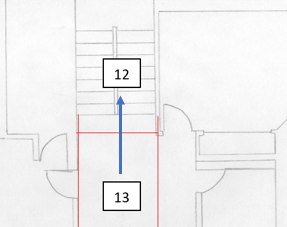
\includegraphics[width=0.5\textwidth]{Imagenes/Evaluacion/del13al8a}}
		& \subfloat[Ruta del cuadrante $11$ al $8$ en la planta baja de la vivienda.]{
			\label{fig:del11al8}
			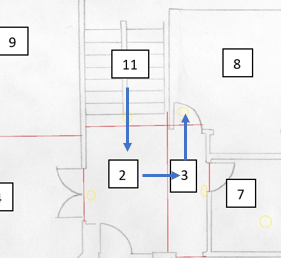
\includegraphics[width=0.5\textwidth]{Imagenes/Evaluacion/del13al8b}}\\
	\end{tabular}
	\caption{Ruta del cuadrante $13$ al $8$.}
	\label{fig:del13al8}
\end{figure}

\subsubsection*{Comportamiento esperado}

Al arrancar la aplicación con el lector de pantalla activado se debe reproducir el nombre de la aplicación (que corresponde con el título de la pantalla inicial) así como el nombre del primer botón (\textit{Iniciar ruta}). Si nos desplazamos con el lector de pantalla por los tres botones existentes debemos escuchar el nombre de cada uno de ellos al posicionarnos encima. Una vez que se ha pulsado \textit{Iniciar ruta} y se despliega la pantalla de destinos debemos escuchar el título de la misma. Con ayuda del lector de pantalla se comprueba que se pueden recorrer todos los botones (incluida la barra de búsqueda y el micrófono) y se introduce el destino ``estancia 8'' por cada uno de ellos, comprobando que no se produce ningún solapamiento de información entre el lector y el \textit{text to speech} utilizado, incluso si el destino no es correcto. Cuando se ha introducido el destino y se pasa a la pantalla de ruta, se comprueba que el usuario recibe la información del cambio de pantalla mediante la lectura del título de la misma y se pueden recorrer todos los botones de la misma manera. Una vez pulsado \textit{Iniciar ruta} las instrucciones comienzan a reproducirse de la manera esperada. Solo en el caso de que, mediante el lector, se cambie de botón se recibe información sobre este. De esta manera, la ejecución continúa de la forma descrita en las pruebas anteriores.  

En cuanto a la generación de instrucciones se refiere, se espera que en el \textit{hall} de la planta baja la primera instrucción de giro (correspondiente al cuadrante $2$) se indique tras avanzar un par de pasos desde el cuadrante $11$. Una vez hecho el giro, el \textit{beacon$3$} debe avisar al usuario del otro giro a la izquierda rápidamente, para permitir que el usuario llegue a su destino de la manera más cómoda posible.

\subsubsection*{Comportamiento durante la prueba}

El arranque de la aplicación con el lector de pantalla activado se realiza de la manera descrita anteriormente. Cabe destacar que en la pantalla de destinos la primera opción que lee el lector de pantalla es el primer botón correspondiente a un destino. Cuando se ha terminado de barrer los botones destino, se lee el de micrófono y el de la barra de búsqueda en ese orden. En la pantalla de ruta el primer botón que se lee es el botón de modo silencio, seguido del resto. Se comprueba el barrido de todos ellos sin ningún comentario relevante y se inicia la ruta. Durante el transcurso de la ruta el lector de pantalla no reproduce nada, debido a que el único cambio que se produce en la interfaz es la actualización del texto correspondiente a las instrucciones y el lector no tiene acceso a él (por implementación). Se comprueba que si se intenta acceder a alguna funcionalidad mientras se está reproduciendo la información asociada a una instrucción, el \textit{text to speech} y el lector de pantalla se solapan. 

A continuación se muestran las instrucciones generadas y el posterior análisis del desarrollo del proceso de guía.

\begin{itemize}
	\item Cuadrante 13: \textit{Continúa recto 5.0 metros.}
	
	\item Cuadrante 12: \textit{El ascensor está delante. Baja a la planta 0.}
	
	\item Cuadrante 11: \textit{Continúa recto 5.0 metros para salir de la zona de ascensores.}
	
	\item Cuadrante 2: \textit{Gira a la izquierda. Luego continúa recto 5.0 metros.}
	
	\item Cuadrante 3: \textit{Gira a la izquierda. Luego continúa recto 5.0 metros.}
	
	\item Cuadrante 8: \textit{Tu destino está delante.}
\end{itemize}


Se observa que la instrucción de giro del cuadrante $2$ tarda demasiado en llegar, haciendo que tengamos que recorrer casi todo el \textit{hall} hasta obtenerla. Esto puede deberse a la aglomeración de \textit{beacons} en esta zona y a que la ubicación del \textit{beacon$2$} favorece que la instrucción de giro hacia el \textit{beacon$3$} se dé con cierto retraso. El final de la ruta se desarrolla de la manera esperada. 

\subsubsection*{Conclusiones}

El problema que surge aquí es que los giros que hay que realizar en la planta baja son bastante tediosos. Por un lado, la ubicación del \textit{beacon$2$} hace que la instrucción de giro hacia el \textit{beacon$3$} tarde demasiado en llegar, puesto que cuando el usuario llega al cuadrante $11$ y avanza queda en mitad del \textit{hall}. Hasta que el usuario no prosigue unos metros, la aplicación no percibe el \textit{beacon$2$} como el más cercano. Una vez que se proporciona la instrucción de giro del cuadrante $2$, el cuadrante $3$ vuelve a hacer girar al usuario hacia el $8$, lo que provoca cierta confusión, por la cantidad de giros seguidos. De igual manera se probó la ruta inversa, desde el cuadrante $8$ al $13$, y el resultado fue análogo.

Gracias a que la implementación de la aplicación está pensada para su utilización con el lector de pantalla activado, el funcionamiento de la misma con (y sin) esta opción no presenta ningún problema, siempre cuando no se utilice el lector para navegar por la pantalla mientras se está reproduciendo una instrucción u otra información asociada a la ejecución de la propia aplicación (la repetición de una instrucción o la activación/desactivación del modo instrucciones detalladas, por ejemplo).


\subsubsection{Ruta del cuadrante $9$ al cuadrante $13$}
\label{subsub:9al13}

Como la ruta por el \textit{hall} de la planta baja había resultado tediosa en el caso anterior, se hizo una prueba desde el otro extremo a fin de establecer si la ubicación de los \textit{beacons} daban lugar a un recorrido más sencillo. En este caso se detalla el comportamiento observado para la ruta con inicio en el cuadrante $9$ y final en el cuadrante $13$ (ver Figura \ref{fig:del9al3}).

\subsubsection*{Objetivos de la prueba}

\begin{itemize}
	\item Observación y evaluación del comportamiento de la aplicación cuando se inicia una ruta que implica un cambio de planta desde los cuadrantes situados en la parte izquierda del mapa.
	\item Comparación de este comportamiento con el observado en la prueba anterior.
\end{itemize}


\subsubsection*{Comportamiento esperado}

En este caso, lo que se quiere es observar cómo se comporta la aplicación en cuanto al momento en el que se indican las instrucciones. En la prueba anterior se pudo ver que la ubicación del \textit{beacon$2$} hace que la instrucción de giro hacia el cuadrante $3$ tarde en llegar cuando se viene del cuadrante $11$. Con esta prueba esperamos obtener la indicación en un momento más adecuado, pues el \textit{beacon$2$} está situado justo en la intersección entre este cuadrante y el $11$.

\begin{figure}[t]
	\centering
	
	\begin{tabular}{cc}
		\subfloat[Ruta del cuadrante $9$ al $11$ en la planta baja de la vivienda.]{
			\label{fig:del9al11}
			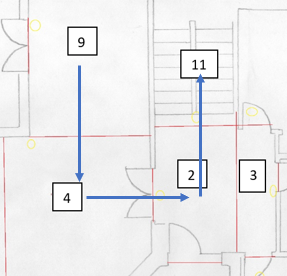
\includegraphics[width=0.5\textwidth]{Imagenes/Evaluacion/del9al11}}
		& \subfloat[Ruta del cuadrante $12$ al $13$ en la planta alta de la vivienda.]{
			\label{fig:del12al13_2}
			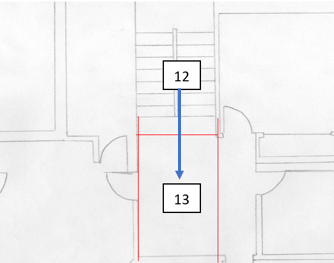
\includegraphics[width=0.5\textwidth]{Imagenes/Evaluacion/del1al13b}}\\
	\end{tabular}
	\caption{Ruta del cuadrante $9$ al $13$.}
	\label{fig:del9al3}
\end{figure}

\subsubsection*{Comportamiento durante la prueba}

Comenzamos exponiendo las instrucciones generadas por la aplicación para discutir posteriormente cómo se ha desarrollado la guía en este caso:

\begin{itemize}
	\item Cuadrante 9: \textit{Continúa recto 5.0 metros. Luego gira a la izquierda.}
	
	\item Cuadrante 4: \textit{Gira a la izquierda. Luego continúa recto 5.0 metros.}
	
	\item Cuadrante 2: \textit{Gira a la izquierda. Luego continúa recto 5.0 metros.}
	
	\item Cuadrante 11: \textit{El ascensor está delante. Sube a la planta 1.}
	
	\item Cuadrante 12: \textit{Continúa recto 5.0 metros para salir de la zona de ascensores.}
	
	\item Cuadrante 13: \textit{Tu destino está delante.}
\end{itemize}


Después del inicio de la ruta en el cuadrante $9$, la indicación de giro a la izquierda del cuadrante $4$ se indicó justo antes de hacer el giro, mejor que en ninguna otra prueba realizada en este cuadrante anteriormente. Tras la llegada a la puerta que separa los cuadrantes $4$ y $2$ la instrucción de giro a la izquierda también fue inmediata. Por su parte, la instrucción del cuadrante $11$ tardó unos tres segundos en darse, una vez que nos ubicamos justo delante de las escaleras. El final de la prueba fue el esperado (ver Sección \ref{subsub:del1al13})

\subsubsection*{Conclusiones}

El hecho de que la instrucción asociada al \textit{beacon$4$} se haya dado con tanta precision esta vez puede deberse a que, en la zona correspondiente al inicio de la ruta, la concentración de \textit{beacons} es mínima.

Esta vez la ubicación del \textit{beacon$2$} favorece el giro del usuario para encontrar el ascensor (escaleras en este caso). De esta manera la ruta resulta mucho más natural y organizada que en el caso anterior. Con esto se pone de manifiesto la importancia del mapeo y la ubicación de los \textit{beacons}.


\subsection{Pruebas de usuario perdido}
\label{sub:usuarioPerdido}

En esta sección se expone el comportamiento de la aplicación en pruebas que simulan que el usuario sale de la ruta correcta.

\subsubsection{Ruta del cuadrante $0$ al cuadrante $10$, eliminando el \textit{beacon} del cuadrante $4$}

En la Sección \ref{subsub:0al10sin4} vimos un caso en el cual era probable que un usuario se desviara de la ruta, debido a la pérdida de la instrucción de giro asociada al cuadrante $4$. En esta ocasión hemos continuado recto a fin de comprobar si la aplicación es capaz de detectar la salida de la ruta por parte del usuario. 

\subsubsection*{Objetivo de la prueba}

\begin{itemize}
	\item Se quiere comprobar que la aplicación es capaz de identificar, en un tiempo razonable, que el usuario se ha salido de la ruta y redirigirlo hacia el destino deseado.
\end{itemize}


\subsubsection*{Comportamiento esperado}

Al perder la instrucción de giro del cuadrante $4$, lo más probable es que el usuario continúe recto hasta llegar al cuadrante $5$ (ver Figura \ref{fig:del0al10sin4perdido}). Si esto ocurre, el comportamiento de la aplicación debería ser el siguiente. Como ya se ha comentado en varias ocasiones, cuando no se detecta como más cercano el \textit{beacon} asociado al siguiente cuadrante de la ruta, la aplicación va contando en una variable \textit{numPasosPerdidos} el número de veces que ha escaneado los \textit{beacons} de su alcance. Cuando esta variable alcanza un umbral y el \textit{beacon} más cercano no corresponde con un \textit{beacon} más avanzado de la ruta, la aplicación interpreta que el usuario se ha salido de la ruta e indica que debe volver por la dirección en la que venía. Desde ese punto le permite iniciar de nuevo la ruta al destino desde su posición actual, pulsando sobre \textit{Iniciar ruta} en la pantalla de ruta. Para la ruta de la Figura \ref{fig:del0al10sin4perdido}, se debería estimar que el usuario se ha perdido cuando llega al cuadrante $5$. En este momento, y tras comenzar la ruta de nuevo hacia la estancia 10, la primera instrucción debería ser ``continúa recto'', pues se presupone que el usuario se ha dado la vuelta como le sugiere la aplicación. A partir de ese momento, la ejecución debe proseguir de la manera descrita en la Sección \ref{subsub:0al10sin4}.

\subsubsection*{Comportamiento durante la prueba}

Exponemos, en primer lugar, las instrucciones que recibió el usuario:

\begin{itemize}
	\item Las instrucciones correspondientes a los cuadrantes del $0$ al $4$ son las mismas que las ya expuestas en la Sección \ref{subsub:0al10}. 
	
	\item Al llegar al cuadrante $5$, el usuario recibe el siguiente aviso: \textit{La dirección tomada no ha sido la correcta. Da la vuelta para volver en la dirección en la que venías. La nueva ruta comenzará cuando pulses Iniciar ruta.} Desde ese punto las instrucciones de guía hasta el cuadrante $10$ se reanudan tomando como origen el cuadrante $5$. 
	
	\item Cuadrante 5: \textit{Continúa recto 5.0 metros. Luego gira a la izquierda.}
	
	\item Las instrucciones correspondientes a los cuadrantes del $4$ al $10$ son las mismas que las ya expuestas en la Sección \ref{subsub:0al10}.
\end{itemize}

Tras recorrer el cuadrante $4$, la aplicación detectó la pérdida del usuario cuando pasaron apenas dos segundos desde que se llegó al cuadrante $5$. Se dieron las indicaciones establecidas y la ruta hacia la estancia 10 comenzó de nuevo al pulsar \textit{Iniciar ruta}. Cabe destacar que el posicionamiento inicial en el cuadrante $5$ se hizo de manera correcta. El final de la ruta se desarrolló de la manera prevista.

\subsubsection*{Conclusiones}

En esta sección hemos podido comprobar otro caso donde el umbral de la variable \textit{numPasosPerdidos} cobra importancia. Es necesario que este se ajuste a las características del mapeo, pues si en un caso como este el umbral hubiera sido muy elevado habríamos estado caminando en la dirección incorrecta demasiado (supongamos que a la izquierda del cuadrante $5$ hubiera más espacio). Como hemos podido comprobar, el ajuste está bien realizado y la aplicación es capaz de determinar con cierta exactitud cuándo un usuario se ha perdido.


\begin{figure}[t!]
	\centering
	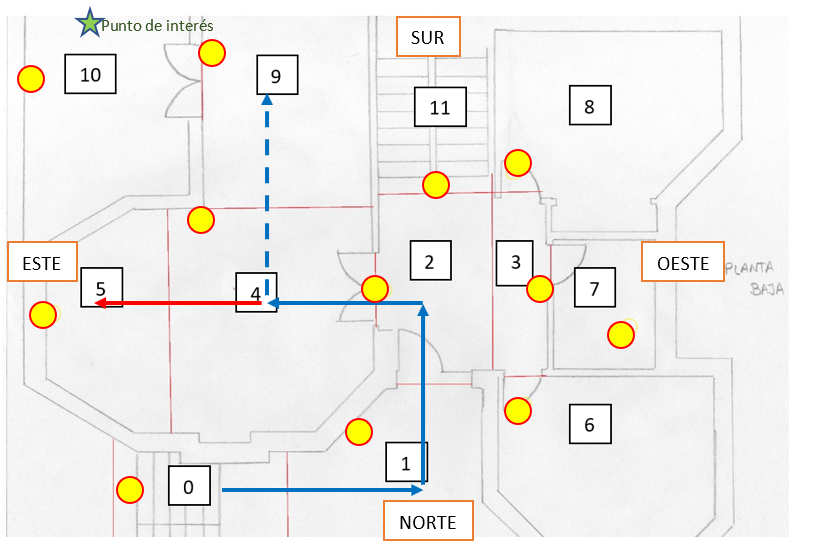
\includegraphics[width=0.8\textwidth]{Imagenes/Evaluacion/del0al10sin4perdido}
	\caption{Ruta del cuadrante $0$ al $10$, donde la instrucción del cuadrante $4$ se ha perdido.}
	\label{fig:del0al10sin4perdido}
\end{figure}


\subsubsection{Usuario fuera del rango de los \textit{beacons}}

Además, la aplicación está preparada para el caso en el que no se detecte ningún \textit{beacon}. Esta situación se reprodujo avanzando hacia la izquierda del cuadrante $0$ y eliminando los \textit{beacons} más próximos a esa zona para provocar que ninguno de ellos fuera detectado.

\subsubsection*{Objetivo de la prueba}

\begin{itemize}
	\item Se quiere comprobar que la aplicación es capaz de identificar la situación en la cual no se detecte ningún \textit{beacon} cerca y advertir al usuario de la misma. 
\end{itemize}

\subsubsection*{Comportamiento esperado}

 Si no se produjera ninguna detección transcurrido un tiempo (determinado por una variable umbral, ver Sección \ref{sub:func_cliente}), la aplicación advierte al usuario de la situación indicándole que debe posicionarse dentro del edificio\footnote{Se asume que si ningún \textit{beacon} es detectado es porque el usuario no se encuentra dentro del edificio o la zona mapeada.} \textit{Te encuentras fuera del alcance de la aplicación. Dirígete al interior del edificio, la ruta comenzará cuando pulses sobre Iniciar ruta.} 
 
\subsubsection*{Comportamiento durante la prueba}

El comportamiento durante la ejecución de esta prueba se corresponde con el comportamiento esperado. El tiempo que tardó la aplicación en advertir al usuario fue relativamente corto, lo que sugiere un posible ajuste de la variable umbral. En cualquier caso, el valor de este umbral no es tan crítico como el umbral relativo al usuario perdido que se ha visto en pruebas anteriores, lo que permite mayor libertad a la hora de asignar una cifra.

\subsubsection*{Conclusiones}

Es importante que la aplicación sea capaz de identificar este tipo de situaciones, pues permiten que el usuario conozca la razón por la cual la aplicación tarda en responder y en indicarle las instrucciones. De esta manera, el usuario descarta que sea un problema de funcionamiento de la aplicación o, incluso, de su propio dispositivo móvil. 


\section{Conclusiones de la evaluación}
\label{sec:conclusionesEval}

En las pruebas realizadas y descritas en la Sección \ref{sec:realizYresult} se ha puesto de manifiesto el comportamiento de la aplicación en situaciones normales y extremas, abordando también aquellos casos en los que el usuario se pierde. En esta sección se exponen los puntos más relevantes obtenidos tras el análisis de las situaciones vistas.


\begin{itemize}
	\item \textit{El código de la aplicación funciona de la manera esperada.} A lo largo de las numerosas rutas de prueba se ha podido comprobar que las instrucciones, vibraciones y sonidos se reproducen e indican al usuario de la manera esperada. No se ha apreciado ningún comportamiento inesperado o erróneo. 
	
	\item \textit{El mapeo del edificio juega un papel primordial.} Como se puede observar en las Secciones \ref{subsub:13al8} y \ref{subsub:9al13} la disposición de los cuadrantes y \textit{beacons} puede facilitar la ruta al usuario en gran medida. Por ello, cuantos menos cuadrantes más sencilla será la ruta. La ubicación de los \textit{beacons} debe ser lo más neutra posible. Es decir, que no favorezca más una ruta que otra.
	
	\item  \textit{Se debe ajustar el umbral de la variable numPasosPerdidos al espacio comprendido entre los beacons.} Han sido varias las ocasiones donde se ha puesto en evidencia la necesidad del ajuste de este umbral. Para asignar el valor del mismo hay que tener en cuenta la distancia entre lo \textit{beacons} y el tiempo que tarda en recorrer ese espacio una persona con discapacidad visual, que suele ser ligeramente mayor que el tiempo que tarda una persona vidente.
	
	\item \textit{La generalidad de la aplicación.} Debido a las circunstancias, la evaluación de la aplicación ha sido realizada en un edificio distinto a la Facultad de Informática de la UCM. Gracias a una implementación general, apenas dependiente del espacio donde se despliega, el esfuerzo para poder adaptarla queda reducido a la realización de los archivos XML y json de la Sección \ref{sec:mapeo}.
	
	\item \textit{Ventajas de las instrucciones e información adicional anticipadas.} Como pudimos ver en la Sección \ref{subsub:1al5sin2}, el hecho de que las instrucciones de giro se avisen con un cuadrante de antelación prepara al usuario para el cambio de dirección, favoreciendo que este no se salga de la ruta, y, en caso de que el \textit{beacon} de la intersección no se detecte, facilita que la información de la ruta persista. Lo mismo ocurre con la información adicional, sobre todo en el caso de los ascensores, pues permite al usuario identificar que debe cambiar de planta para llegar a su destino por adelantado.

\end{itemize}

A pesar de que no ha sido detallado expresamente durante la realización de las pruebas, hay que mencionar que el resto de funcionalidades como la lectura y reproducción de las instrucciones del modo de uso de la aplicación o distintas pruebas con el micrófono y la barra de búsqueda para diferentes destinos, también fueron comprobados, sin destacar ningún comportamiento extraño o inesperado.

